%%%%%%%%%%%%%%%%%%%%%%%%%%%%%%%%%%%%%%%%%
% Beamer Presentation
% LaTeX Template
% Version 1.0 (10/11/12)
%
% This template has been downloaded from:
% http://www.LaTeXTemplates.com
%
% License:
% CC BY-NC-SA 3.0 (http://creativecommons.org/licenses/by-nc-sa/3.0/)
%
%%%%%%%%%%%%%%%%%%%%%%%%%%%%%%%%%%%%%%%%%

%----------------------------------------------------------------------------------------
%	PACKAGES AND THEMES
%----------------------------------------------------------------------------------------

\documentclass{beamer}

\mode<presentation> {

% The Beamer class comes with a number of default slide themes
% which change the colors and layouts of slides. Below this is a list
% of all the themes, uncomment each in turn to see what they look like.

%\usetheme{default}
%\usetheme{AnnArbor}
%\usetheme{Antibes}
%\usetheme{Bergen}
%\usetheme{Berkeley}
%\usetheme{Berlin}
%\usetheme{Boadilla}
%\usetheme{CambridgeUS}
%\usetheme{Copenhagen}
%\usetheme{Darmstadt}
%\usetheme{Dresden}
%\usetheme{Frankfurt}
%\usetheme{Goettingen}
%\usetheme{Hannover}
%\usetheme{Ilmenau}
%\usetheme{JuanLesPins}
%\usetheme{Luebeck}
\usetheme{Madrid}
%\usetheme{Malmoe}
%\usetheme{Marburg}
%\usetheme{Montpellier}
%\usetheme{PaloAlto}
%\usetheme{Pittsburgh}
%\usetheme{Rochester}
%\usetheme{Singapore}
%\usetheme{Szeged}
%\usetheme{Warsaw}

% As well as themes, the Beamer class has a number of color themes
% for any slide theme. Uncomment each of these in turn to see how it
% changes the colors of your current slide theme.

%\usecolortheme{albatross}
%\usecolortheme{beaver}
%\usecolortheme{beetle}
%\usecolortheme{crane}
%\usecolortheme{dolphin}
%\usecolortheme{dove}
%\usecolortheme{fly}
%\usecolortheme{lily}
%\usecolortheme{orchid}
%\usecolortheme{rose}
%\usecolortheme{seagull}
%\usecolortheme{seahorse}
%\usecolortheme{whale}
%\usecolortheme{wolverine}

%\setbeamertemplate{footline} % To remove the footer line in all slides uncomment this line
%\setbeamertemplate{footline}[page number] % To replace the footer line in all slides with a simple slide count uncomment this line

%\setbeamertemplate{navigation symbols}{} % To remove the navigation symbols from the bottom of all slides uncomment this line
}

\usepackage{graphicx} % Allows including images
\usepackage{booktabs} % Allows the use of \toprule, \midrule and \bottomrule in tables

\setbeamercovered{transparent}

%----------------------------------------------------------------------------------------
%	TITLE PAGE
%----------------------------------------------------------------------------------------

\title[Cardano \& the Cubic]{Cardano and the Cubic Equation} % The short title appears at the bottom of every slide, the full title is only on the title page

\author{Ben Sepanski} % Your name
\date{\today} % Date, can be changed to a custom date

\begin{document}

\begin{frame}
\titlepage % Print the title page as the first slide
\end{frame}

% thanks slide
\begin{frame}
\frametitle{Special Thanks}
Thanks to Dr. Markus Hunziker for the book recommendation, and to
William Dunham, whose chapter {\it Cardano and the Solution of the
Cubic} in the book {\it Journey through Genius} provided the primary
source for this talk.
\end{frame}

\begin{frame}
\frametitle{Overview} % Table of contents slide, comment this block out to remove it
\tableofcontents % Throughout your presentation, if you choose to use \section{} and \subsection{} commands, these will automatically be printed on this slide as an overview of your presentation
\end{frame}

%----------------------------------------------------------------------------------------
%	PRESENTATION SLIDES
%----------------------------------------------------------------------------------------

%------------------------------------------------
\section{A Teensy Bit of (Unfortunately) Math} 
%------------------------------------------------

\subsection{What is a cubic?}

\begin{frame}
\frametitle{Solving for $x$}
\begin{block}{Linear Equation}
\begin{equation}
    mx + b = 0
\end{equation}
\end{block}
i.e., solve equations that look like this (easy): 
\begin{equation*}
    3x + 2 = 0,\qquad
    x - 5 = 0,\qquad
    42 x - 123456789 =0 
\end{equation*}

\uncover<2->{
    \begin{block}{Quadratic Equation}
    \begin{equation}
        ax^2 + bx + c = 0
    \end{equation}
    \end{block}
    i.e., solve equations that look like this (only a little harder): 
    \begin{equation*}
        2x^2+3x + 2 = 0,\qquad
        4x^2+x - 5 = 0,\qquad
        -123x^2+42 x - 123456789 =0 
    \end{equation*}
}
\end{frame}

%%%%%%%%%%%%%%%%%%%%%%%%%%%%%%%%%%%%%%%%%%%%%%%%%%%%%%%%%%%%%%%%%%%%%%
%%%%%%%%%%%%%%%%%%%%%%%%%%%%%%%%%%%%%%%%%%%%%%%%%%%%%%%%%%%%%%%%%%%%%%

\begin{frame}
\frametitle{Solving for $x$}
What's the natural next equation to solve? \emph{The cubic:}
\begin{block}{Cubic Equation}
\begin{equation}
    ax^3 + bx^2+cx+d = 0
\end{equation}
\end{block}
i.e., solve equations that look like this (hard): 
\begin{eqnarray*}
    4x^3-2x^3+3x + 2 = 0,\\
    100x^3 + x - 5 = 0,\\
    42x^3 - 21x^2+42 x - 123456789 =0 
\end{eqnarray*}

\end{frame}

%%%%%%%%%%%%%%%%%%%%%%%%%%%%%%%%%%%%%%%%%%%%%%%%%%%%%%%%%%%%%%%%%%%%%%
%%%%%%%%%%%%%%%%%%%%%%%%%%%%%%%%%%%%%%%%%%%%%%%%%%%%%%%%%%%%%%%%%%%%%%

\subsection{Luca Pacioli's {\it Summa de Arithmetica}} 
\begin{frame}
\frametitle{{\it Summa de Arithmetica}}

\begin{columns}[c]
\column{.45\textwidth}
\begin{block}{Luca Pacioli (1494)}
    In a contemporary mathematics textbook, Pacioli assesses solving the cubic
    equation as impossible as ``squaring the circle", a problem posed by
    the ancient Greeks (and proven impossible in the 1800s).
\end{block}

\column{.5\textwidth}
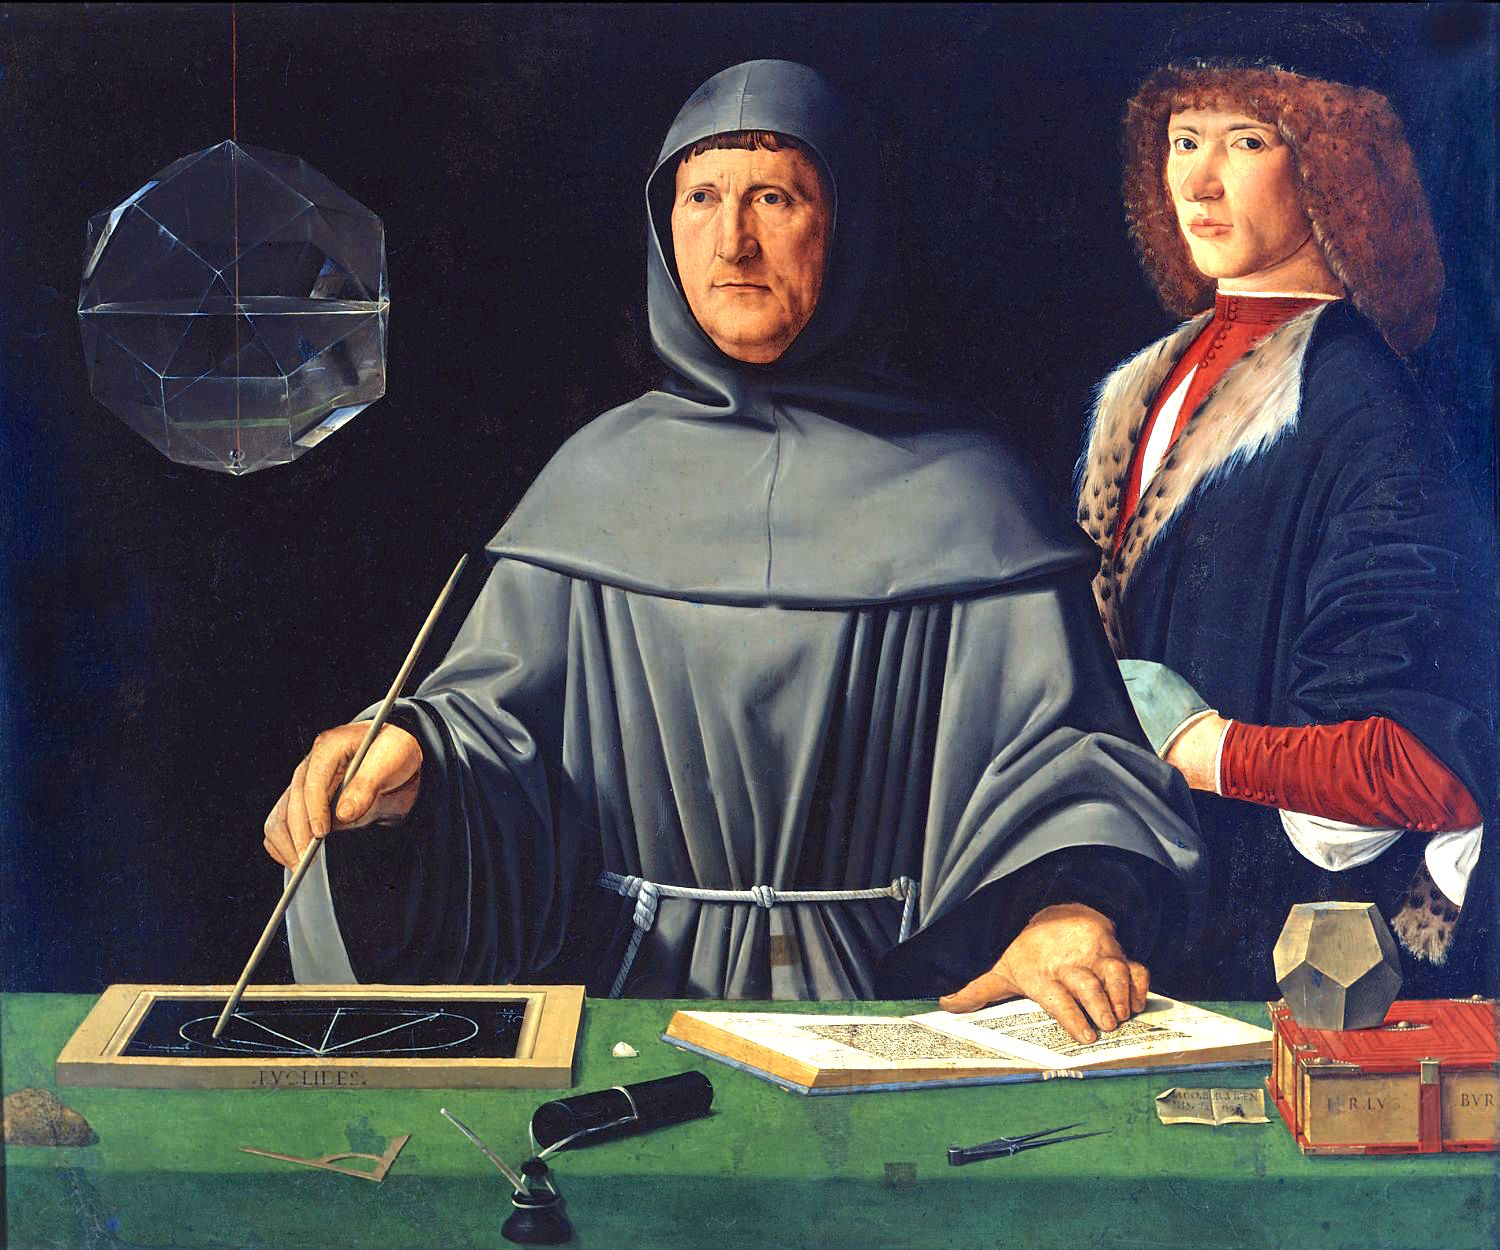
\includegraphics[width=\textwidth]{Luca-Pacioli}\\[-1ex]
{\tiny Source: from \emph{Wikipedia}, painting often attributed to Jacopo
de'Barbari, 1495 }
\end{columns}
\end{frame}

%%%%%%%%%%%%%%%%%%%%%%%%%%%%%%%%%%%%%%%%%%%%%%%%%%%%%%%%%%%%%%%%%%%%%%
%%%%%%%%%%%%%%%%%%%%%%%%%%%%%%%%%%%%%%%%%%%%%%%%%%%%%%%%%%%%%%%%%%%%%%

\section{Rising Action}
\subsection{del Ferro, Fior, \& Tartaglia}
\begin{frame}
\frametitle{del Ferro \& Fior}

\begin{itemize}
    \item
    This all changed, when Scipione del Ferro solves the ``repressed cubic:"
    \begin{equation*}
        x^3 + mx = n
    \end{equation*}
    \item
    But, he kept the solution secret.
    \item On his deathbed in 1526, del Ferro tells his student, Antonio
    Fior
    \item A hothead, Fior challenges a noted scholar--Niccolo Fontana
\end{itemize}
\end{frame}

%%%%%%%%%%%%%%%%%%%%%%%%%%%%%%%%%%%%%%%%%%%%%%%%%%%%%%%%%%%%%%%%%%%%%%
%%%%%%%%%%%%%%%%%%%%%%%%%%%%%%%%%%%%%%%%%%%%%%%%%%%%%%%%%%%%%%%%%%%%%%

\begin{frame}
\frametitle{Tartaglia}
\begin{columns}[c]
\column{.45\textwidth}
\only<1>{
\begin{block}{Tartaglia (1499-1557)}
    \begin{itemize}
    \item
    Niccolo Fontana, better known as ``Tartaglia" (meaning ``the
    Stammerer", due to a war wound).

    \item
    Fontana had boasted he could solve cubics of another form.
    \end{itemize}
\end{block}
}

\only<2>{
\begin{block}{The Challenge}
    \begin{itemize}
    \item
    Fior gives Tartaglia 30 ``repressed cubics", Tartaglia gave Fior 30
    problems of various topics.

    \item
    Working furiously, Tartaglia discovers the solution the night before
    the problems are due, winning 30 to 0.

    \item 
    Fior fades from history.
    \end{itemize}
\end{block}
}

\column{.5\textwidth}
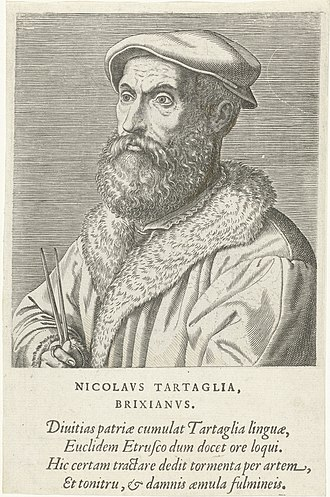
\includegraphics[width=\textwidth]{Tartaglia}\\[-1ex]
{\tiny Source: from \emph{Wikipedia}}
\end{columns}
\end{frame}

%%%%%%%%%%%%%%%%%%%%%%%%%%%%%%%%%%%%%%%%%%%%%%%%%%%%%%%%%%%%%%%%%%%%%%
%%%%%%%%%%%%%%%%%%%%%%%%%%%%%%%%%%%%%%%%%%%%%%%%%%%%%%%%%%%%%%%%%%%%%%

\subsection{Cardano \& Ferrari}

%%%%%%%%%%%%%%%%%%%%%%%%%%%%%%%%%%%%%%%%%%%%%%%%%%%%%%%%%%%%%%%%%%%%%%
%%%%%%%%%%%%%%%%%%%%%%%%%%%%%%%%%%%%%%%%%%%%%%%%%%%%%%%%%%%%%%%%%%%%%%
\begin{frame}
\frametitle{Cardano}
\begin{columns}
    \column{.5\textwidth}
    \only<1>{
    Now enters the strangest character of the story--Gerolamo Cardano
    (1501-1576). His story is a half-hour talk, so we proceed with a
    negligent survey.
    }

    \only<2>
    {
    \begin{block}{Cardano--Ups and Downs}
        \begin{itemize}
            \item A failed and successful doctor with severe
            psychological issues (he loved the feeling of pain
            \emph{ending})
            \item An avid gambler and one of the first statisticians
            \item Father of a murderer
            \item Stellar mathematician, ardent astrologer
            \item Author of a (dubious) autobiography
            \item Arrested for heresy, held a pension from the Pope
        \end{itemize}
    \end{block}
    }

    \column{.5\textwidth}
    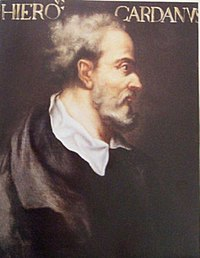
\includegraphics[width=\textwidth]{Gerolamo-Cardano}\\[-1ex]
    {\tiny Source: from \emph{Wikipedia}}
\end{columns}
\end{frame}

%%%%%%%%%%%%%%%%%%%%%%%%%%%%%%%%%%%%%%%%%%%%%%%%%%%%%%%%%%%%%%%%%%%%%%
%%%%%%%%%%%%%%%%%%%%%%%%%%%%%%%%%%%%%%%%%%%%%%%%%%%%%%%%%%%%%%%%%%%%%%

\begin{frame}
\frametitle{Ferrari}
\begin{columns}[c]
\column{.5\textwidth}
\vfill
\begin{itemize}
    \item
    Enter the final player in our story--Ludovico Ferrari.
    
    \vspace{8mm}

    \item 
    {\it Ars Magna} (``Great Art")

    \vspace{8mm}

    \item
    To include the solution of the cubic, begged Tartaglia.
\end{itemize}

\column{.5\textwidth}

\begin{block}{Ferrari (1522-1565)}
\begin{itemize}
    \item Asked for work from Cardano--on the very day Cardano had
    received a good omen (the incessant squawking of a magpie)
    
    \item Quickly turned to his colleague, by the age of 20 Ferrari was
    a near equal
\end{itemize}
\end{block}

\end{columns}
\end{frame}

%%%%%%%%%%%%%%%%%%%%%%%%%%%%%%%%%%%%%%%%%%%%%%%%%%%%%%%%%%%%%%%%%%%%%%
%%%%%%%%%%%%%%%%%%%%%%%%%%%%%%%%%%%%%%%%%%%%%%%%%%%%%%%%%%%%%%%%%%%%%%

\section{Fallout}
\subsection{Tartaglia Relents}

\begin{frame}
\frametitle{Tartaglia's Conditions}
\begin{itemize}
    \uncover<1->{\item
        After much begging, Tartaglia gives Cardano the solution--in the
        form of a poem
        \begin{itemize}
            \item Ferrari uses the ideas to solve the ``next"
            equation--the quartic!
        \end{itemize}
        \vspace{5mm}
        \item
        The equation must be kept encoded
    }
        \vspace{5mm}
    \uncover<2->{\item
        This won't do for Cardano--he wants to put it in a book!
        \vspace{5mm}
        \item
        Suddenly, Cardano and Ferrari have an idea.
    }
\end{itemize}
\end{frame}

%%%%%%%%%%%%%%%%%%%%%%%%%%%%%%%%%%%%%%%%%%%%%%%%%%%%%%%%%%%%%%%%%%%%%%
%%%%%%%%%%%%%%%%%%%%%%%%%%%%%%%%%%%%%%%%%%%%%%%%%%%%%%%%%%%%%%%%%%%%%%

\begin{frame}
\frametitle{Sneaking Around}
\begin{itemize}
    \item Remember del Ferro?
    \begin{itemize}
        \vspace{5mm}
        \item Cardano and Ferrari do
        \vspace{5mm}
        \item Obtaining the solution (identical to Tartaglia's) from del
        Ferro's notes, Cardano and Ferrari publish.
        \vspace{5mm}
        \item del Ferro is credited.
    \end{itemize}
\end{itemize}
\end{frame}

%%%%%%%%%%%%%%%%%%%%%%%%%%%%%%%%%%%%%%%%%%%%%%%%%%%%%%%%%%%%%%%%%%%%%%
%%%%%%%%%%%%%%%%%%%%%%%%%%%%%%%%%%%%%%%%%%%%%%%%%%%%%%%%%%%%%%%%%%%%%%

\subsection{Tartaglia Challenges}

\begin{frame}
\frametitle{Backlash from Tartaglia}
\begin{itemize}
    \uncover<1->{
    \item Accusations and insults fly back and forth between Tartaglia
    and Ferrari (rather a hot-head)
    }

    \vspace{3mm}

    \uncover<2->{
    \item A contest ensues on Ferrari's home turf
    \begin{itemize}
        \item Cardano does not even show
    \end{itemize}
    }

    \vspace{3mm}

    \uncover<3->{
    \item Tartaglia loses--blaming the ``rowdiness and partisanship of
    the crowd"
    \begin{itemize}
        \item Given Ferrari's reputation, some historians believe he was
        lucky to escape with his life.
    \end{itemize}
    }
\end{itemize}
\end{frame}
%%%%%%%%%%%%%%%%%%%%%%%%%%%%%%%%%%%%%%%%%%%%%%%%%%%%%%%%%%%%%%%%%%%%%%
%%%%%%%%%%%%%%%%%%%%%%%%%%%%%%%%%%%%%%%%%%%%%%%%%%%%%%%%%%%%%%%%%%%%%%

%------------------------------------------------

\begin{frame}
\Huge{\centerline{The End}}
\end{frame}

%----------------------------------------------------------------------------------------

\end{document} 
